\chapter{Implementation in das DietrichOnline-Projekt}

In diesem Kapitel wird die Implementation ins DietrichOnline-Projekt genauer erläutert.

\section{Vorbereitung}

Um den Elasticsearch-Klienten zu nutzen, muss dieser zuerst einmal per Composer installiert werden. Die geschieht durch einen Eintrag in die composer.json.

Um für den nun folgenden Vergleich ein faires Spielfeld aufzubauen, wurde eine Datenbank, welche auf demselben Server wie Elasticsearch liegt verwendet. So ist sichergestellt, dass die Verbindung zum Server für beide Parteien gleich ist.

Zum Testen wird nun zuerst die Lemma-Abfrage, in einer modifizierten Fassung \ref{lemmaIndexierungEla}, verwendet.

Durch die eben aktivierte X-Security von Elasticsearch braucht der Klient diesmal einen Zugang per API-Key. Dieser kann mithilfe eines Curl Befehls generiert werden \ref{lst:elaApi}. Der API-Key bekommt hierbei lesende Rechte auf alle Dietrich-Indices. Auch muss die Zertifikats-Autorität bei jeder Anfrage mitgegeben werden. 

\begin{lstlisting}[language=JSON, frame=single, label={lst:elaApi}] 
POST /_security/api_key
{
  "name": "dietrich-website",
  "role_descriptors": { 
    "role-a": {
      "cluster": ["all"],
      "index": [
        {
          "names": ["dietrich_*"],
          "privileges": ["read"]
        }
      ]
}}}
\end{lstlisting}


\subsubsection{Indexierung}
\label{lemmaIndexierungEla}

Um nun alle Daten in richtiger Form in das Projekt zu laden, muss die Indexierung von damals umgeschrieben werden. 

Bei den Joins wurden M zu N Beziehungen auf eine flache Ebene gezogen. Dabei wird der Eintrag so oft abgebildet, wie es Objekte in der M zu N Beziehung gibt. 

Zur Verdeutlichung hier ein Beispiel.
Es gibt eine Tabelle Artikel, welche eine M zu N Beziehung mit der Tabelle DDC bezieht. In der Artikel Tabelle gibt es den Eintrag Trier mit der ID 1, der mit 2 DDC Einträgen, Trier und Rheinland-Pfalz verbunden wird. Bei einem Join wird nun alles in eine flache Hierachie gezogen. Deswegen würde die Tabelle der Ergebnisse des Joins nun die Folgenden Einträge enthalten \ref{tbl:join}.

\begin{table} %[hbtp]
	\centering
		\begin{tabular}{l | l | l}
		    \textbf{ID} & \textbf{Artikel} & \textbf{DDC} \\
        \hline
        01 & Trier & Trier \\
        01 & Trier & Rheinland-Pflaz  \\
		\end{tabular}
    \caption{Tabelle für ein Beispiel der Joins}
    \label{tbl:join}
\end{table}

Um nun einen solchen Eintrag in Elasticsearch abzubilden wird ein Array in Elasticsearch benötigt. Für solche Fälle gibt es den Aggregat-Filter in Logstash. Dieser aggregiert auf Basis der ID die Daten. So ist es nun möglich Code zu schreiben, der automatisch die Daten in Arrays zusammenfasst.

Dabei ist es wichtig, dass dieser Prozess nicht in mehreren Threads ausgeführt wird. Daher erhält jede Pipeline in diesem Projekt auch maximal einen Thread.
Hier nun einmal ein Beispiel aus dem Code \ref{lst:fronendConf}.


\begin{lstlisting}[language=Ruby, frame=single, label={lst:fronendConf}] 
[...]
map['bstatus_beschreibung'] ||= event.get('bstatus_beschreibung')

map['ddc_entries'] ||= []
if event.get('ddc_notation') != nil
    duplicate = false
    map['ddc_entries'].each { |n|
        if n.value?(event.get('ddc_notation'))
            duplicate = true
            break
        end
    }
    if !duplicate
        map['ddc_entries'] << {
            'ddc_notation' => event.get('ddc_notation'),
            'ddc_schlagwort' => event.get('ddc_schlagwort'),
            'ddc_webdewey_is_checked' => 
              event.get('ddc_webdewey_is_checked')
        }
    end
end
[...]
\end{lstlisting}

Dieser Code wird nun so lange in einer Schleife durchlaufen, wie dieselbe ID aus der Datenbank kommt. Der Wert bstatus\_beschreibung wird dabei zum Beispiel bei jeden Durchlauf überschrieben. 

Damit die sich ändernden Wert aggregiert werden, wurde ein Code geschrieben, welche Einträge in eine Array schreibt. Da bei dieser Abfrage \ref{lst:sqlQuery} nun allerdings mehrere Lefts Joins aufeinander ausgeführt werden, kann es dazu kommen, das sich Zeilen wiederholen. Um dieses Problem zu lösen wurde ein Code geschrieben der Duplikate und NULL Werte erkennt und nicht nochmals in das Array einträgt.

\section{Aufbau der Abfrage}

Als SQL-Framework wurde Doctrine verwendet. Dieses bietet eine Abstraktion für SQL in Objekte. Im Hintergrund werden diese Objekte dann in SQL übersetzt. Die hier betrachtete Abfrage wurde schonmal von Hand optimiert, da zuerst alle Ids der anzuzeigenden Lemmata gesucht werden, und erst im zweiten Schritt alle Joins auf den verbleibenden Datensätzen ausgeführt werden.

Die Elasticsearch-Abfrage anderseits besteht nur aus einer Abfrage, da hier alle Daten schon auf einer flachen Ebene existieren.

Verwendet wird hier ein sogenannter Boolean-Query. Dieser enthält vier verschieden Untergruppierungen.

Zuerst einmal der Must-Teil. Alle hier Angegeben Parameter müssen in jedem Ergebnis vorhanden sein. Dies ist gleichzustellen mit einem booleschen AND. 

Als Zweites der Must-Not-Teil. Dieser Teil ist den Must-Teil sehr ähnlich, allerdings sind die Parameter negiert.

Danach der Shoud-Teil. In diesem Teil muss nur einer der Parameter vorhanden sein. Dies ist zu vergleichen mit einem booleschen OR. 

Und zuletzt der Filter-Teil. Die gesetzten Filter sind auch Must-Befehle. Allerdings werden diese nicht bei der Gewichtung der Ergebnisse mit eingerechnet. Für diese Arbeit hat dies erstmal keinen Einfluss, da alle Ergebnisse alphabetisch sortiert werden. Daher ist diese Abfrage mit Must gleichzustellen. \cite{ElasticsearchB.V..17.12.2019}


\begin{lstlisting}[language=PHP, frame=single, label={lst:queryEla}] 
//Create Client with basic Params
$mustNotQueries = [];
$filters        = [];
$mustQueries    = [];

if ($character === LemmaEntity::NOT_A_TO_Z_CHARACTER) {
    $mustQueries[] = ['regexp' => ['bezeichnung.keyword' => 
      ['value' => '@&~(^[a-zA-Z].+)', 'flags' => 'ALL']]];
      
    $filters[]     = ['term' => ['ist_geloescht' => false]];
} elseif ($character === LemmaEntity::DELETED) {
    $filters[] = ['term' => ['ist_geloescht' => true]];
} else {
    $mustQueries = ['prefix' => ['bezeichnung.keyword' => "$character"]];
    $filters[]   = ['term' => ['ist_geloescht' => false]];
}

switch ($filter) {
    case self::STATUS_FILTER_KLAR:
        $filters[] = ['term' => ['bstatusbezeichnung' => 'klar']];
        break;
    //[Other Filters]
}

$params['body']['query']['bool']['must']     = $mustQueries;
$params['body']['query']['bool']['must_not'] = $mustNotQueries;
$params['body']['query']['bool']['filter']   = $filters;

return $client->search($params)['hits']['hits'];
\end{lstlisting}

In Zeile 14 ist hier zu sehen, dass anstelle der Wildcard-Abfrage, welcher in der vorherigen Abfrage \ref{lst:phpElastic} verwendet wurde, ein Prefix-Abfrage verwendet wird. Dieser bietet eine sauberere Lösung zum Suchen von Wortanfängen.

\section{Vergleich}

Die oben beschriebenen Abfragen wurden jetzt jeweils 100-Mal mit einem Timer laufen gelassen. 

Bei dem Vergleich kamen die folgenden Durchschnittswerte zustande:
\begin{table} %[hbtp]
	\centering
		\begin{tabular}{l | l }
		    \textbf{System} & \textbf{Zeit} \\
        \hline
        MariaDB + Doctrine & 3.49 \\
        Elasticsearch      & 1.45  \\
		\end{tabular}
    \caption{Vergleich der Laufzeit zur Abfrage aller Daten für Buchstabe S der Lemma-Administration (15.846 Einträge)}
    \label{vlgTimeDBvsEla}
\end{table}

Dabei ist zu sehen, dass Elasticsearch eine Reduktion der Zeit um 58,45 \% ermöglicht.

Diese Abfrage wurde auch noch in einer nachgebauten Produktionsumgebung ausgeführt. Daran erkennt man, dass die Abfrage durchaus schneller agiert, allerdings im Gesamtkontext kaum einen Unterschied macht. Elasticsearch lädt mit 46,49 Sekunden durchaus als Doctrine mit 50,1 Sekunden, allerdings fällt dies bei der langen Ladezeit kaum ins Gewicht.


\begin{figure}
	\centering
	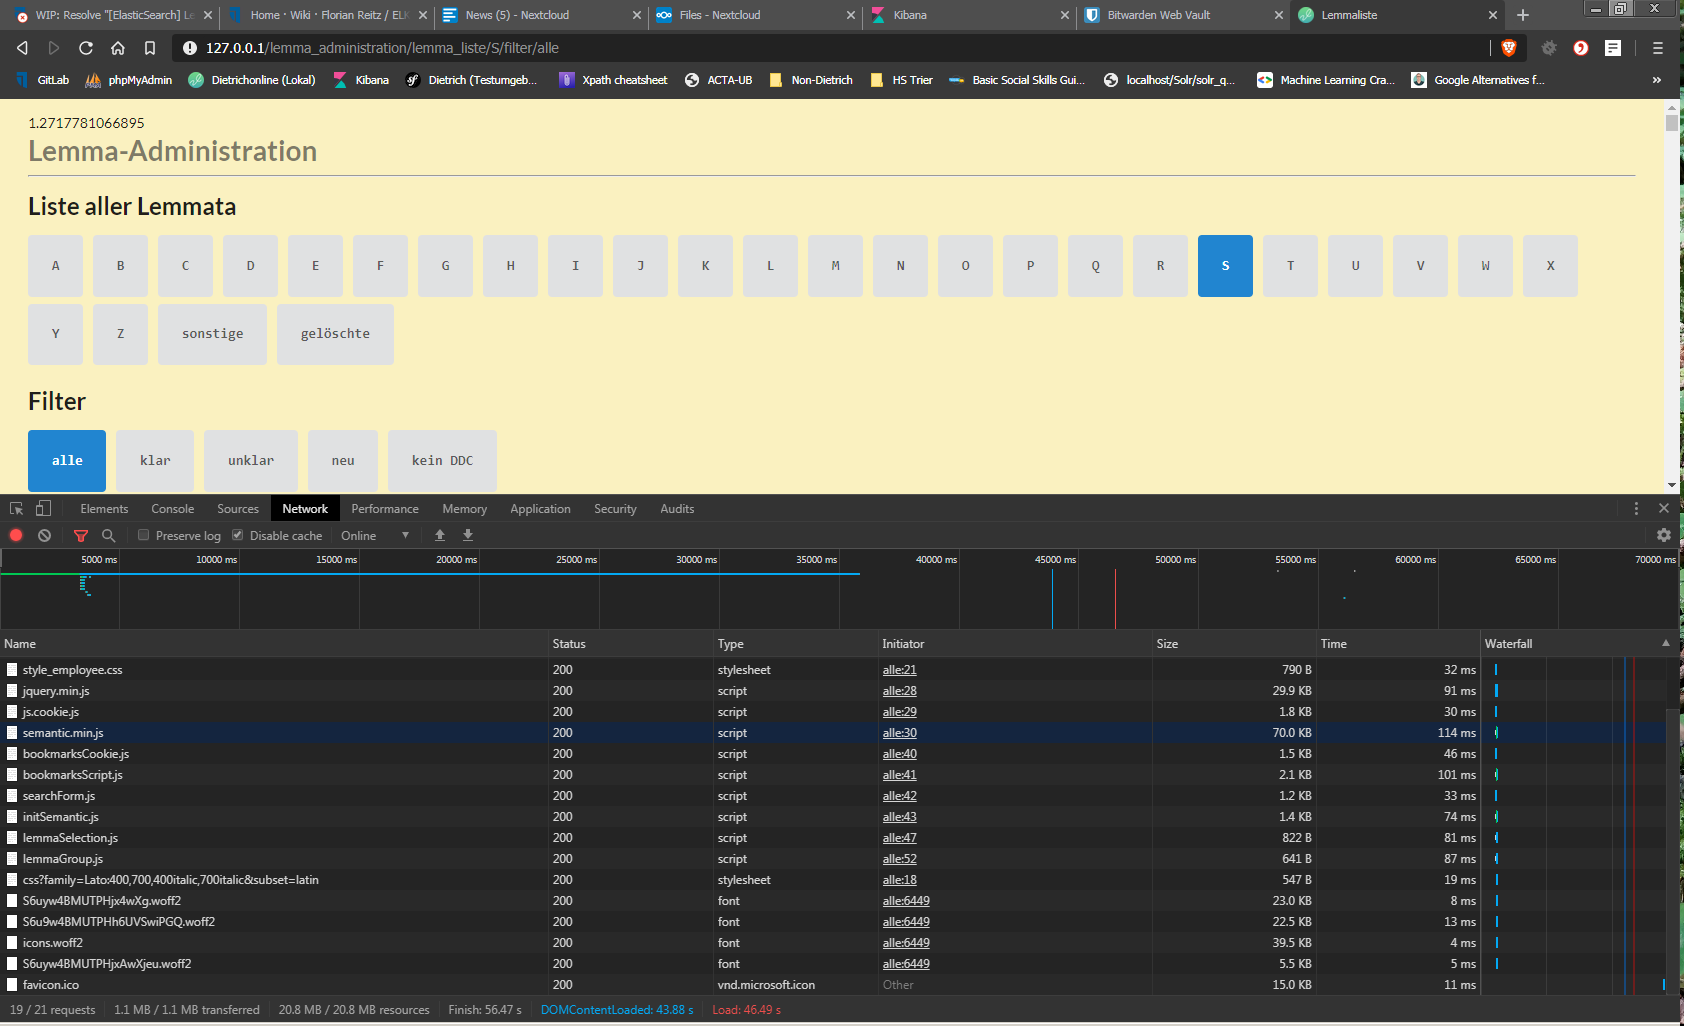
\includegraphics[width=1\linewidth]{images/setup/query/time_prod_ela.png}
	\caption{Query-Geschwindigkeit: Elasticsearch}
	\label{img:timeProdEla}
\end{figure}

\begin{figure}
	\centering
	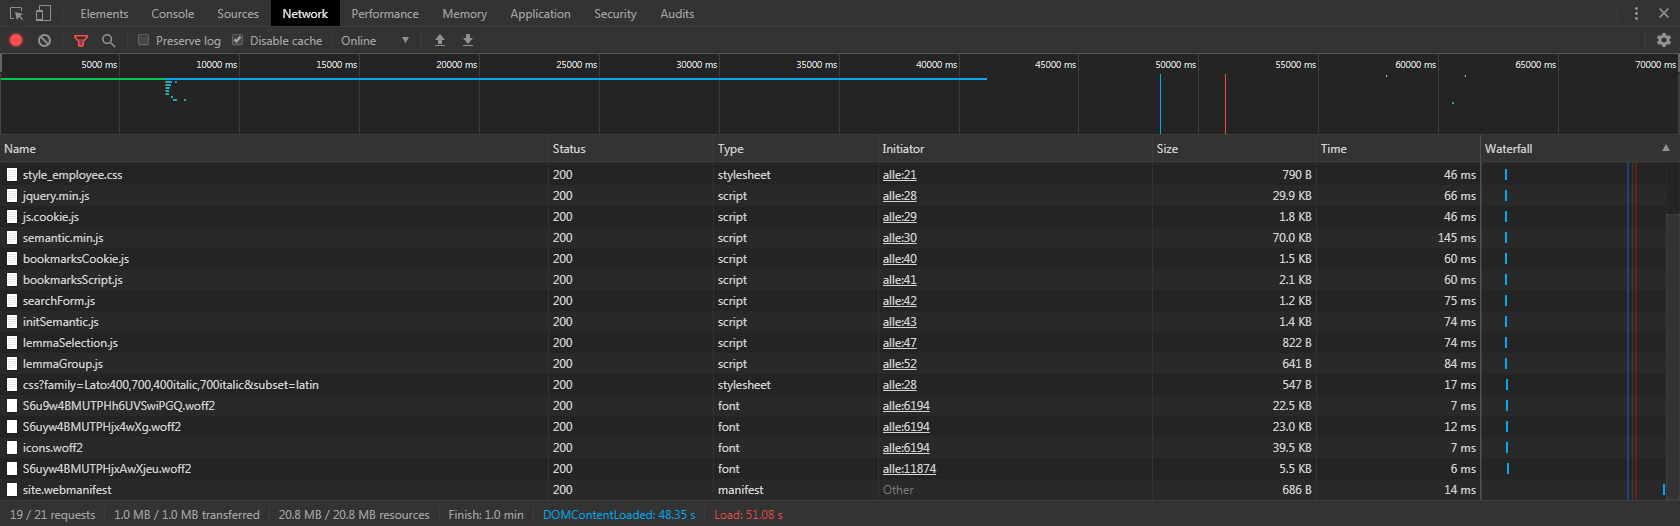
\includegraphics[width=1\linewidth]{images/setup/query/time_prod_db.png}
	\caption{Query-Geschwindigkeit: Doctrine}
	\label{img:timeProdDb}
\end{figure}

